\documentclass[article]{rian_article}

%%
% Atenção: Compilar com pdflatex !!!
%%

% Para colocar ao lado use \And para quebrar a linha use \AND
\author{Rian G.S. Pinheiro\\ \email{rian@ic.ufal.br}\And 
        Eric Coelho\\ \email{esc2@ic.ufal.br}}% \And
%         Terceiro Autor\\ \email{terceiro@ic.ufal.br} \AND
%         Quarto Autor\\ \email{quarto@ic.ufal.br} \And
%         Quinto Autor\\ \email{quinto@ic.ufal.br}}

% Autores separados por \&, se mais que 3 usar et al.
\Plainauthor{Rian Pinheiro \& Eric Coelho} %% comma-separated


\title{Algoritmo Genético BRKGA para o Problema de Empacotamento 2D 	Clássico com desempate}
\Plaintitle{Algoritmo Genético BRKGA para o Problema de Empacotamento 2D Clássico com desempate} %% Titulo sem formatação
\Shorttitle{BRKGA com desempate} %% a short title (aparece no topo das páginas)


%% an abstract and keywords
\Abstract{
	O \textit{Problema de empacotamento} (BPP) consiste em armazenar ortogonalmente um conjunto de itens na menor quantidade de caixas possível. A versão clássica assume que os itens têm orientação fixa e não pode haver sobreposição no empacotamento. O caso bidimensional generaliza o problema de empacotamento unidimensional clássico amplamente difundido na literatura, portanto, é da classe \NPhard~.
	Este trabalho apresenta um algoritmo genético de chaves aleatórias viciadas (BRKGA) para o \textit{problema de empacotamento bidimensional} (2BP), considerando os itens alocados com orientação fixa, baseando-se em chaves aleatórias como critério de desempate entre os espaços vazios ao inserir um novo item. O problema tem várias aplicações industriais, como corte, repartição e agendamento, relacionando-se a outros problemas complexos.
}

\Keywords{BRKGA, Bin Packing, 2BP, Meta-heurísticas}
\Plainkeywords{BRKGA, Bin Packing, 2BP, Meta-heurísticas} %% sem formatação


%% Informações do Trabalho
\Versao{1}
% \Versao{Final}
\Year{2020}
\Semestre{2}
\Month{Fevereiro}
\Submitdate{\today}
\Disciplina{Pesquisa Operacional}


%%%%%%%%%%%%%%%%%%%%%%%%%% PACOTES %%%%%%%%%%%%%%%%%%%%%%%%%%
\usepackage{amsmath}
\usepackage{bbm}
\usepackage{float}
\usepackage{subfig}
\usepackage{indentfirst}
\usepackage[T1]{fontenc}
\usepackage{url,bm}
\usepackage{textcomp}
\usepackage{graphicx}
\usepackage{amssymb}
\usepackage{anysize}
\usepackage{algpseudocode}
\usepackage{algorithm}
\usepackage{amsthm}
\usepackage{tikz}
\usepackage{enumerate}

%%%%%%%%%%%%%%%%%%%%%%%%% Comandos %%%%%%%%%%%%%%%%%%%%%%%%%%%%
\newcommand{\Cpp}{C\nolinebreak\hspace{-.05em}\raisebox{.4ex}{\tiny\bf +}\nolinebreak\hspace{-.10em}\raisebox{.4ex}{\tiny\bf +}~} 
\newcommand{\NPcom}{$\mathcal{NP}$-completo}
\newcommand{\NPhard}{$\mathcal{NP}$-Difícil}
\newtheorem{teorema}{Teorema}[section]
\floatname{algorithm}{Algoritmo}
\newenvironment{prova}{\begin{proof}[\bf\textsc{Prova.}]}{\end{proof}}



\begin{document}

% Este exemplo foi publicado no SBPO 2015.
\section{Introdução}

O \textit{problema de empacotamento clássico bidimensional} (2BP) consiste em empacotar ortogonalmente um conjunto de $n$ itens em forma de retângulos caracterizados por sua altura $h_{i}$ e largura $w_{i}$, $i \in \{1, 2, 3, ... , n\}$, no menor número possível de caixas homogêneas de altura $H \geq hi$ e largura $W \geq wi$. A quantidade de caixas é ilimitada e os itens não podem ser alocados com sobreposição.

\begin{figure}[hbt]
\centering
\subfloat[Instância.]{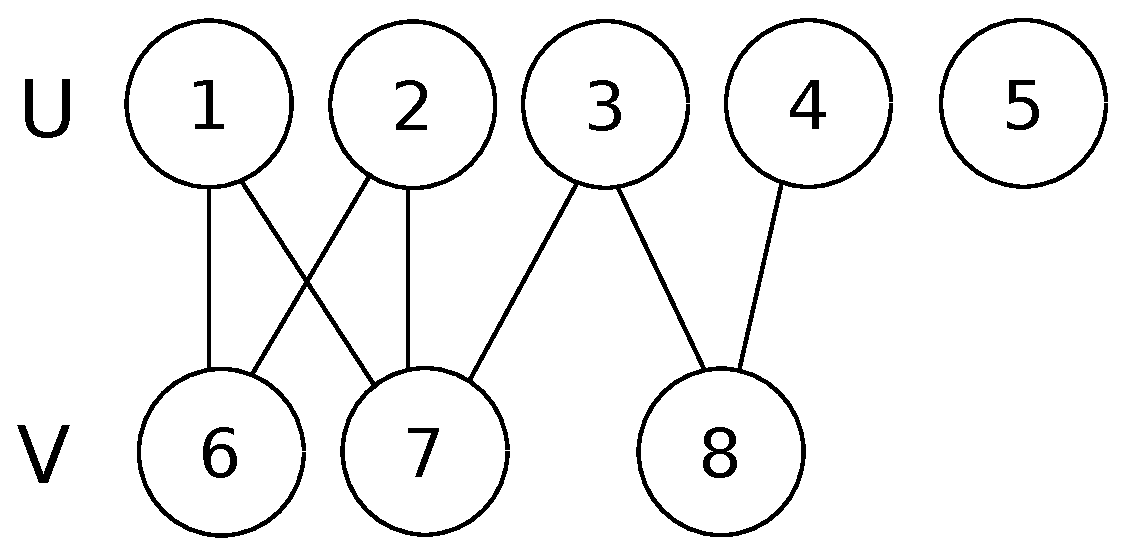
\includegraphics[width=0.3\textwidth]{figs/ex_fig1.eps}}\hspace{0.1\textwidth}
\subfloat[Solução.]{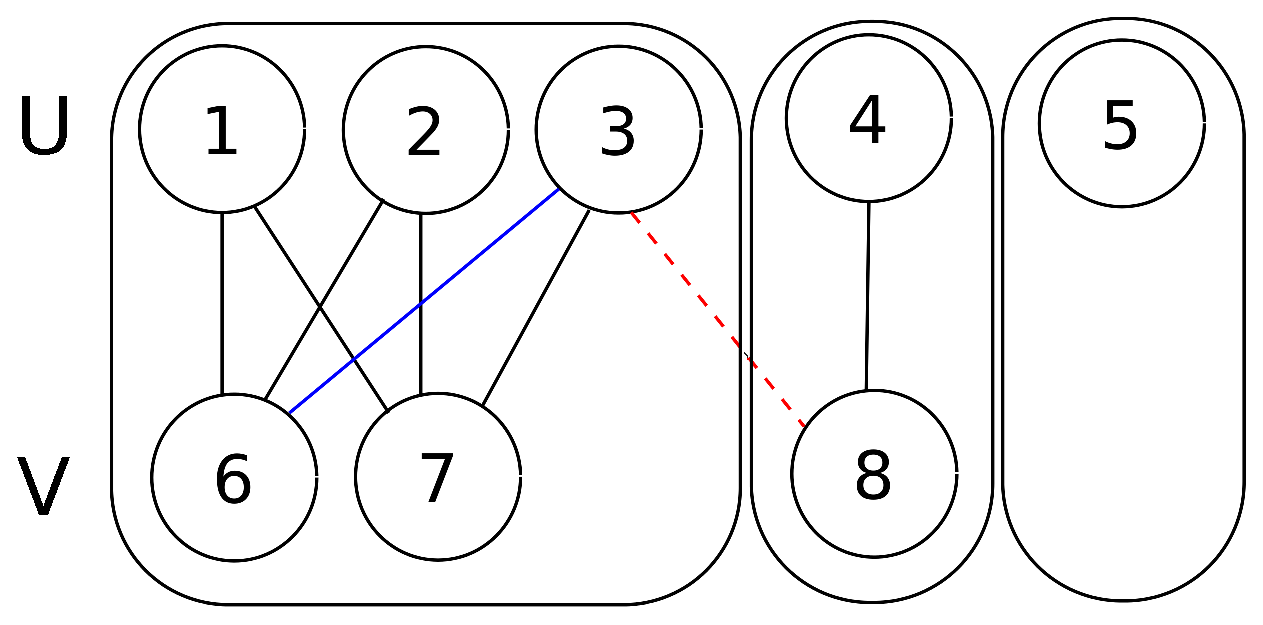
\includegraphics[width=0.33\textwidth]{figs/ex_fig2.eps}}
\caption{Exemplo do BGEP.} \label{fig:ex}
\end{figure}
 
A Figura~\ref{fig:ex} mostra um exemplo de um grafo que com uma adição, aresta $(3,6)$

\subsection{Aplicações}
empty
\section{Algoritmo BRKGA}\label{sec:corte}
O algoritmo genético de chaves aleatórias viciadas (BRKGA) foi introduzido por \citet{resende2013} para problemas de otimização combinatória. Esta meta-heurística é uma variante do algoritmo genético de chaves aleatórias (RKGA) [Bean, 1994]. A ideia principal é evoluir uma população codificada. Os indivíduos são representados por cromossomos, denominado chaves aleatórias ou random-keys, na forma de vetores de números reais no intervalo [0, 1]. A implementação desse processo requer um componente chamado decodificador. Este componente deve receber um vetor de random-keys para fornecer uma representação do indivíduo que pode ser avaliada. O decodificador é o único componente que depende das características do problema. Assim, duas implementações da meta-heurística para diferentes problemas só necessitam de decodificadores diferentes. Para o 2BP, o decodificador é composto de dois componentes: um método de ordenação e um algoritmo guloso para realizar o empacotamento dos itens. Tal algoritmo guloso constrói uma solução iterativamente, recebendo uma permutação de inteiros que representa a sequência em que os itens serão empacotados sequencialmente. O método de ordenação deve receber um vetor com n random-keys, um para cada item da instância, para fornecer uma permutação de itens. As chaves devem ser ordenadas de modo que o item ai é empacotado antes do item aj se e somente se $k_{i} < k_{j}, {i}, {j} \in \{1, ..., {n}\}$, onde $k_{i}$ e $k_{j}$ são as respectivas random-keys associadas.

Após o processo de ordenação, a permutação associada ao cromossomo do indivíduo é passada como parâmetro de entrada para o algoritmo guloso, denominado Distance to the Front-Top-Right Corner (DFTRC). Sabendo que uma caixa aberta da solução corrente é uma que contém itens empacotados, para cada iteração k do DFTRC, procuramos em cada caixa aberta por áreas que podem conter o respectivo item $a_{k}, {k} \in \{1, ..., {n}\}$. Se nenhuma caixa aberta até o momento pode conter o item, então uma nova caixa é introduzida na solução com $a_{k}$ empacotado. No passo de empacotamento, áreas maximais são utilizadas para modelar o espaço vazio de cada caixa aberta. Uma área maximal é a maior área retangular possível dentro da caixa aberta que não há itens. Todas as áreas maximais que podem conter o item da iteração corrente são candidatas para a escolha da localização do empacotamento. O DFTRC seleciona a área maximal que maximiza a distância entre o canto superior direito frontal do item para o respectivo canto superior direito frontal da caixa.

Caso haja empate entre as áreas maximais, um segundo vetor de random keys é utilizado para selecionar entre as duas melhores áreas maximais.


O Algoritmo~\ref{alg:geral} apresenta a visão geral da heurística.

\begin{figure}[hbtp]\centering
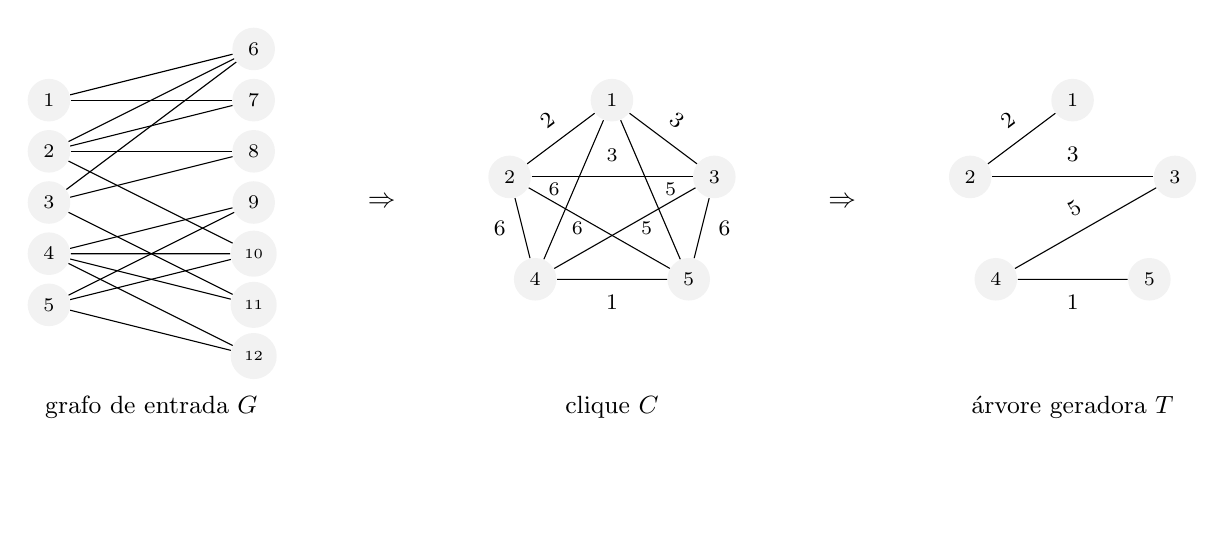
\begin{tikzpicture} [scale=1.3, auto=left,every node/.style={circle,fill=gray!10}]
\node (u2) at (0,0){\scriptsize 1};
\node (u3) at (0,-0.5){\scriptsize 2};
\node (u5) at (0,-1){\scriptsize 3};

\node (u1) at (0,-1.5){\scriptsize 4};
\node (u4) at (0,-2){\scriptsize 5};

\node (v1) at (2,0.5){\scriptsize 6};
\node (v3) at (2,0){\scriptsize 7};
\node (v7) at (2,-0.5){\scriptsize 8};

\node (v2) at (2,-1){\scriptsize 9};
\node (v6) at (2,-1.5){\tiny 10};
\node (v5) at (2,-2){\tiny 11};
\node (v4) at (2,-2.5){\tiny 12};

\foreach \from/\to in {u1/v2,u1/v4,u1/v5,u1/v6,u2/v1,u2/v3,u3/v1,u3/v3,u3/v6,u3/v7,u4/v2,u4/v4,u4/v6,u5/v1,u5/v5,u5/v7}
\draw (\from) -- (\to);

\node[draw=none,fill=none] (label1) at (1,-3) {\small grafo de entrada $G$};

% \pause

\node (c1) at (5.5,0){\scriptsize 1};
\node (c2) at (4.5,-0.75){\scriptsize 2};
\node (c3) at (6.5,-0.75){\scriptsize 3};
\node (c4) at (4.75,-1.75){\scriptsize 4};
\node (c5) at (6.25,-1.75){\scriptsize 5};

\draw (c1) -- (c2) node[fill=none,midway,above,sloped] {\footnotesize 2};
\draw (c1) -- (c3) node[fill=none,midway,above,sloped] {\footnotesize 3};
\draw (c1) -- (c4) node[fill=none,midway,left] {\scriptsize ~~~6};
\draw (c1) -- (c5) node[fill=none,midway,right] {\scriptsize 5~~~};
\draw (c2) -- (c3) node[fill=none,midway,above] {\scriptsize 3};
\draw (c2) -- (c4) node[fill=none,midway,left] {\footnotesize 6};
\draw (c2) -- (c5) node[fill=none,midway,left] {\scriptsize 6};
\draw (c3) -- (c4) node[fill=none,midway,right] {\scriptsize 5};
\draw (c3) -- (c5) node[fill=none,midway,right] {\footnotesize 6};
\draw (c4) -- (c5) node[fill=none,midway,below] {\footnotesize 1};

\node[draw=none,fill=none] (seta1) at (3.25,-1) {$\Rightarrow$};
\node[draw=none,fill=none] (label2) at (5.5,-3) {\small clique $C$};

% \pause

\node (t1) at (10,0){\scriptsize 1};
\node (t2) at (9,-0.75){\scriptsize 2};
\node (t3) at (11,-0.75){\scriptsize 3};
\node (t4) at (9.25,-1.75){\scriptsize 4};
\node (t5) at (10.75,-1.75){\scriptsize 5};

\draw (t1) -- (t2) node[fill=none,midway,above,sloped] {\footnotesize 2};
\draw (t2) -- (t3) node[fill=none,midway,above] {\footnotesize 3};
\draw (t3) -- (t4) node[fill=none,midway,above,sloped] {\footnotesize 5};
\draw (t4) -- (t5) node[fill=none,midway,below] {\footnotesize 1};

\node[draw=none,fill=none] (set2) at (7.75,-1) {$\Rightarrow$};
\node[draw=none,fill=none] (label3) at (10,-3) {\small árvore geradora $T$};

\end{tikzpicture}
\caption{Execução do Algoritmo Construtivo}
\label{fig:construtivo}
\end{figure}

\subsection{Método Construtivo} \label{sec::construtivo}

Dado como entrada a árvore geradora mínima $T$, as soluções iniciais de cada iteração do GRASP são construídas com base em remoções aleatórias das arestas desta árvore.
Na floresta geradora resultante, cada árvore definirá um agrupamento $U_i$ para compor a biclique.

Com base nisso, para cada vértice em $V$, verifica-se em qual agrupamento $U_i$ deverá fazer parte, de maneira a conter o menor número de edições.
Isto é feito associando o vértice em questão a cada uma dos conjuntos de $U_i$ e verificando o quanto de remoções e adições de arestas são necessárias para que esse vértice se ligue com todos os vértices do conjunto associado.

O agrupamento $U_i$ em que seja necessário o menor número de edições será o ideal e portanto escolhido.
Em seguida, combinamos $U$ e $V$ para formarmos a biclusterização $\{U,V\}$ ligando as arestas no grafo $G$.
No algoritmo~\ref{alg:const} apresentamos o método construtivo.

\begin{algorithm}[hbtp]
\caption{Método Construtivo}
\label{alg:const}
\begin{algorithmic}[1]
\footnotesize
\Procedure{Construtivo}{$T,k$}
 \While{$E(T) \neq \emptyset$}
  \State{$\mu \gets \{\infty,\cdots,\infty\}_{1 \times |E(T)|}$}
  \ForAll{$i \in E(T)$}
   \State{$T_i \gets T - \{i\}$}
   \State{construa $U_i$ a partir de $T_i$} \Comment{um biclique para cada componente conexa de $T_i$}
   \State{construa $V_i$ ideal a partir de $U_i$} \Comment{$V_i$ que tem menor número de erros dado $U_i$}
   \State{$C_i \gets$ \textsc{BiCluster}($U_i,V_i$)} \Comment{combina os agrupamentos $U_i$ e $V_i$ para gerar a biclique $C_i$}
   \State{$\mu_{i} \gets$ \textsc{NumEdicoes}($C_i$)}
  \EndFor
  \State{escolha $\tilde{C}$ aleatoriamente entre os $k$ melhores $C_i$} \Comment{baseado nos valores em $\mu$}
  \State{atualiza $T$ com base no $\tilde{C}$ escolhido}
  \If{$\tilde{\mu} < \mu^{\ast} $}
   \State{$C^{\ast} \gets \tilde{C}$}
  \EndIf
 \EndWhile
 \State{\Return{$C^{\ast}$}}
\EndProcedure
\end{algorithmic}
\end{algorithm}

\subsection{Busca Local} \label{sec::buscalocal}
Após o método construtivo, inicia-se o método de Busca Local baseado no VND \citep{martello2002}.
Tendo como entrada um solução inicial, a Busca Local tenta melhorar a solução através da exploração do espaço de solução.
Dado um conjunto de estruturas de vizinhança, o método de Busca Local explora o espaço de solução trocando sistematicamente as estruturas de vizinhança.
O método aceita somente soluções que melhorem a solução corrente.
Nestes casos, o método volta à primeira estrutura de vizinhança e inicia uma nova busca.
Usamos aqui uma variante do VND que consiste em usar uma ordenação aleatória dessas estruturas, como mostrado no Algoritmo~\ref{alg:rvnd}.

O método proposto utiliza três estruturas de vizinhança: ``Reagrupe''; ``Mude de Biclique'' e ``Troca de Vértice''.
A complexidade computacional da busca em cada uma dessas vizinhanças é de $O(n^2)$.
Elas são presentadas a seguir.

\begin{description}
 \item [Reagrupe:]
Dado os conjuntos de grupos de vértices, formados pela intersecção de cada uma das partes, $U$ por exemplo, com cada biclique $B$ da solução atual.
A Busca Local Reagrupe aloca os vértices da outra parte, no caso $V$, ao grupo de vértice de forma a minimizar o número de edições.
 
 \item [Muda de Biclique:]
Esta Busca Local move um vértice de uma biclique para outra.
 
 \item[Troca de Vértice:]
Esta Busca Local troca dois vértices (de mesma parte) de uma biclique para a outra. Ao contrário da ``Mude de Biclique'' não possibilita a eliminação de bicliques previamente existentes.
\end{description}


\begin{algorithm}[htbp]
\caption{VND com ordem aleatórias}
\label{alg:rvnd}
\footnotesize
\begin{algorithmic}[1]
\Procedure{VND}{$A$}
 \State{inicialize $V$ randomicamente}
 \State{$k \gets 1$}
 \State{$\mu^{\ast} \gets \mu(A)$}
 \Repeat 
  \State{$A' \gets V^{k}(A)$} 
  \If{$\mu(A') > \mu^{\ast}$} 
   \State{$A^{\ast} \gets A'$}
   \State{$k \gets 1$}
  \Else
   \State{$k \gets k + 1$}
  \EndIf
 \Until{$k = k_{max}$}
 \State{\Return{$A^{\ast}$}}
\EndProcedure
\end{algorithmic}
\end{algorithm}

\begin{algorithm}[htbp]
\caption{Visão Geral da Heurística GRASP}
\label{alg:geral}
\begin{algorithmic}[1]
\footnotesize
\Procedure{MST+BL}{$G,k$}
 \State{$it \gets 0$}
 \State{$\mu^{\ast} \gets \infty$}
 \State{transforme o grafo $G$ numa clique $C$ com pesos $d_{ij}$}
 \State{calcule a árvore geradora de custo mínimo $T$ de $C$}
 \Repeat 
  \State{$C_{it} \gets$ \textsc{Construtivo}($T,k$)} \Comment{$k = 1$, guloso; $k = m$, aleatório; $1 < k < m$, $k$-melhores}
  \State{$C'_{it} \gets$ \textsc{BuscaLocal}($C_{it}$)} 
  \State{$\mu_{it} \gets$ \textsc{NumEdicoes}($C'_{it}$)} \Comment{número de edições (remoção ou adição de arestas)}
  \If{$\mu_{it} < \mu^{\ast}$} 
   \State{$C^{\ast} \gets C'_{it}$}
  \EndIf
  \State{$it \gets it + 1$}
 \Until{$it = 100$}% + (k - 1) \cdot m$}
 \State{\Return{$C^{\ast}$}}
\EndProcedure
\end{algorithmic}
\end{algorithm}

\section{Experimentos Computacionais}
A base de testes utilizada neste trabalho é composta por 500 instâncias do 2BP detalhadas em \citet{martello1998}. As instâncias são organizadas em 10 classes com 10 instâncias para cada quantidade de itens ${n} \in \{20, 40, 60, 80, 100\}$. Esta base se trata de uma extensão das instâncias propostas em \citet{wang1987}.

\subsection{Ferramentas}\label{sec::ferramentas}

O BRKGA proposto foi implementado utilizando a linguagem de programação C++11, e foi compilado com o GCC do GNU Compiler Collection. O ambiente computacional utilizado em todos os testes neste trabalho consiste de um desktop munido da seguinte configuração: processador AMD FX-6300 @3.5 GHz, 8 GB de memória RAM e sistema operacional Ubuntu 18.04. A Tabela 1 relaciona os parâmetros calibráveis do BRKGA com os respectivos valores.


\subsection{Resultado}

TABELA de RESULTADOS DA EXECUÇÃO

A Tabela~\ref{tab:grasp} apresenta a instância, seguida do número de edições encontradas pelo algoritmo exato \citet{martello2002}, a solução encontrada na literatura \citep{chan1997}, juntamente com a solução do GRASP proposto e do GRASP+SP.
Observa-se que o algoritmo GRASP encontra o valor ótimo em todas as instâncias com exceção da \texttt{i11}.
Já o GRASP+SP, encontrou a solução ótima em todas as instâncias.

\begin{table}[htb]
\caption{Resultados do GRASP e GRASP+SP}
\label{tab:grasp}
\centering
\footnotesize
\begin{tabular}{|l|c|c|c|c|}
\hline
Instância	&Exato    &\citep{chan1997}    & GRASP	& GRASP+SP	\\ \hline
i1	        &17       &17	  & 17		&17		\\ \hline
i2	        &20       &20	  & 20		&20		\\ \hline
i3	        &36       &36	  & 36		&36		\\ \hline
i4	        &34       &34	  & 34		&34		\\ \hline
i5	        &35       &36	  & 35		&35		\\ \hline
i6	        &30       &30	  & 30		&30		\\ \hline
i7	        &50       &51	  & 50		&50		\\ \hline
i8	        &28       &28	  & 28		&28		\\ \hline
i9	        &34       &34	  & 34		&34		\\ \hline
i10	        &52       &53	  & 52		&52		\\ \hline
i11	        &53       &54	  & 54		&\textbf{53}	\\ \hline
i12	        &61       &62	  & 61		&61		\\ \hline
i13	        &54       &54	  & 54		&54		\\ \hline
i14	        &63       &64	  & 63		&63		\\ \hline
i15	        &61       &61	  & 61		&61		\\ \hline
i16         	& 26	  & 28	  & 26		& 26		\\ \hline
i17         	& 40	  & 40	  & 40		& 40		\\ \hline
i18         	& 34	  & 35	  & 34		& 34		\\ \hline
i19         	& 49	  & 49	  & 49		& 49		\\ \hline
i20         	& 51	  & 52	  & 51		& 51		\\ \hline
i21         	& 88	  & 88	  & 88		& 88		\\ \hline
i22         	& 74	  & 74	  & 74		& 74		\\ \hline
i23         	& 24	  & 24	  & 24		& 24		\\ \hline
i24         	& 24	  & 24	  & 24		& 24		\\ \hline
i25         	& 94	  & 94	  & 94		& 94		\\ \hline
i26         	& 23	  & 23	  & 23		& 23		\\ \hline
i27         	& 111	  & 111	  & 111		& 111		\\ \hline
i28         	& 62	  & 63	  & 62		& 62		\\ \hline
i29         	& 56	  & 56	  & 56		& 56		\\ \hline
i30         	& 97	  & 97	  & 97		& 97		\\ \hline
\end{tabular}
\end{table}
 
A Tabela~\ref{tab:tempo} apresenta a instância, junto com o tempo de execução do algoritmo de \citet{martello2002}, o tempo de execução do GRASP proposto e o tempo de execução do GRASP+SP.
Note que, o tempo de GRASP proposto foi muito inferior ao tempo de execução da literatura.
Observa-se ainda que os tempos do GRASP e do GRASP+SP foram próximos.
Além disso, algoritmo de foi executado em uma máquina Intel Core i7-2600 com 3.40GHz, enquanto que o deste artigo foi executado em uma máquina Intel Core i7-4500U com 1.80GHz.


No que diz respeito ao pré-processamento da Seção~\ref{sec:corte}, ele se mostrou eficaz em instâncias esparsas, porém sem muita efetividade para as instâncias densas.

 \begin{table}[hbtp]
\caption{Tempos do GRASP e GRASP+SP}
\label{tab:tempo}
\centering
\footnotesize
\begin{tabular}{|l|c|c|c|}
\hline
Instância	  & \citep{zudio2018}	&GRASP    & GRASP+SP	   \\ \hline
i1	  & 7,23	&0,26	  & 0,30	  \\ \hline 
i2	  & 7,00	&0,21	  & 0,24	  \\ \hline 
i3	  & 10,09	&0,39	  & 0,45	  \\ \hline 
i4	  & 9,97	&0,35  	  & 0,41	  \\ \hline 
i5	  & 12,90	&0,41     & 0,46	  \\ \hline 
i6	  & 13,89	&0,48     & 0,49	  \\ \hline 
i7	  & 7,88	&0,49     & 0,52	  \\ \hline 
i8	  & 13,13	&0,39     & 0,42	  \\ \hline 
i9	  & 12,53	&0,47     & 0,50	  \\ \hline 
i10	  & 20,31	&0,98     & 1,09	  \\ \hline 
i11	  & 23,41	&1,35     & 1,17	  \\ \hline 
i12	  & 24,50	&1,40     & 1,26	  \\ \hline 
i13	  & 47,19	&2,66	  & 2,39	  \\ \hline 
i14	  & 48,24	&2,82	  & 2,78	  \\ \hline 
i15	  & 65,95	&3,27	  & 3,25	  \\ \hline
i16  	& 3,40		& 0,09	   & 0,10	  \\ \hline
i17  	& 4,02		& 0,05	   &  0,05	  \\ \hline
i18  	& 5,26		& 0,12	   &  0,14	  \\ \hline
i19  	& 5,28		& 0,06	   &  0,08	  \\ \hline
i20  	& 7,05		& 0,36	   &  0,39	  \\ \hline
i21  	& 31,80		& 0,15	   &  0,14	  \\ \hline
i22  	& 24,27		& 0,17	   &  0,14	  \\ \hline
i23  	& 26,45		& 1,71	   &  1,48	  \\ \hline
i24  	& 25,56		& 3,28	   &  3,24	  \\ \hline
i25  	& 26,48		& 0,16	   &  0,19	  \\ \hline
i26  	& 43,42		& 2,95	   &  3,05	  \\ \hline
i27  	& 51,80		& 0,20	   &  0,22        \\ \hline
i28  	& 77,30		& 15,52	   &  16,09	  \\ \hline
i29  	& 71,91		& 13,73	   &  13,65	  \\ \hline
i30  	& 77,21		& 0,34	   &  0,37	  \\ \hline
\end{tabular}
\end{table}


\section{Conclusão}
Este trabalho aplicou a heurística BRKGA para o problema clássico de empacotamento bidimensional, sem considerar a rotação dos itens. O algoritmo é baseado na meta-heurística BRKGA, e utiliza um algoritmo guloso para empacotar os itens. Através de um conjunto de 500 instâncias, as quais compõem a base de teste padrão para vários trabalhos encontrados na literatura, o BRKGA foi comparado com outras abordagens encontradas na literatura. Os experimentos mostraram que o BRKGA proposto aliado com o critério de desempate obtém resultados equivalentes ou melhores aos reportados na literatura.

PROPROSTAS
Para trabalhos futuros serão propostas novas melhorias que acelerem o método, como por exemplo novo módulos exatos.
Pretende-se estender o pré-processamento proposto para os coasos em que a biclique não é completa.
Além disso, um estudo mais aprofundado com relação à elaboração de instâncias mais difíceis.
Com relação a meta-heurística, pode-se pensar em novos métodos construtivos e novas buscas locais.


\bibliography{refs2}
\end{document}
